\documentclass[degree=master]{thuthesis}
% 选项:
%   degree=[bachelor|master|doctor|postdoctor], % 必选
%   secret,                                     % 可选
%   pifootnote,                                 % 可选(建议打开)
%   openany|openright,                          % 可选,基本不用
%   arial,                                      % 可选,基本不用
%   arialtoc,                                   % 可选,基本不用
%   arialtitle                                  % 可选,基本不用

% 所有其它可能用到的包都统一放到这里了,可以根据自己的实际添加或者删除。
\usepackage{thuthesis}

% 定义所有的图片文件在 figures 子目录下
\graphicspath{{figures/}}

% 可以在这里修改配置文件中的定义。导言区可以使用中文。
% \def\myname{薛瑞尼}

\begin{document}

%%% 封面部分
\frontmatter
\thusetup{
  %******************************
  % 注意:
  %   1. 配置里面不要出现空行
  %   2. 不需要的配置信息可以删除
  %******************************
  %
  %=====
  % 秘级
  %=====
  secretlevel={秘密},
  secretyear={10},
  %
  %=========
  % 中文信息
  %=========
  ctitle={基于Vive VR的遥操作机械手},
  cdegree={工学硕士},
  cdepartment={天空工场},
  cmajor={计算机科学与技术},
  cauthor={薛瑞尼},
  csupervisor={郑纬民教授},
  cassosupervisor={陈文光教授}, % 副指导老师
  ccosupervisor={某某某教授}, % 联合指导老师
  % 日期自动使用当前时间,若需指定按如下方式修改:
  % cdate={超新星纪元},
  %
  % 博士后专有部分
  cfirstdiscipline={计算机科学与技术},
  cseconddiscipline={系统结构},
  postdoctordate={2009年7月——2011年7月},
  id={编号}, % 可以留空: id={},
  udc={UDC}, % 可以留空
  catalognumber={分类号}, % 可以留空
  %
  %=========
  % 英文信息
  %=========
  etitle={An Introduction to \LaTeX{} Thesis Template of Tsinghua University v\version},
  % 这块比较复杂,需要分情况讨论:
  % 1. 学术型硕士
  %    edegree:必须为Master of Arts或Master of Science(注意大小写)
  %             “哲学、文学、历史学、法学、教育学、艺术学门类,公共管理学科
  %              填写Master of Arts,其它填写Master of Science”
  %    emajor:“获得一级学科授权的学科填写一级学科名称,其它填写二级学科名称”
  % 2. 专业型硕士
  %    edegree:“填写专业学位英文名称全称”
  %    emajor:“工程硕士填写工程领域,其它专业学位不填写此项”
  % 3. 学术型博士
  %    edegree:Doctor of Philosophy(注意大小写)
  %    emajor:“获得一级学科授权的学科填写一级学科名称,其它填写二级学科名称”
  % 4. 专业型博士
  %    edegree:“填写专业学位英文名称全称”
  %    emajor:不填写此项
  edegree={Doctor of Engineering},
  emajor={Computer Science and Technology},
  eauthor={Xue Ruini},
  esupervisor={Professor Zheng Weimin},
  eassosupervisor={Chen Wenguang},
  % 日期自动生成,若需指定按如下方式修改:
  % edate={December, 2005}
  %
  % 关键词用“英文逗号”分割
  ckeywords={机器人, 虚拟现实, 远程控制},
  ekeywords={\TeX, \LaTeX, CJK, template, thesis}
}

% 定义中英文摘要和关键字
\begin{cabstract}
随着机器人技术的发展,机器人的应用场景越来越多。但是目前自动控制机器人尚不能执行多数复杂任务,特别是抢险救灾等需要随机应变的任务,这种情况下需要遥操作机器人。

目前机械臂远程控制普遍采用手柄或键盘控制方式,且监控方式普遍为摄像头图像显示在监视器上,与现场操作差别很大。我们开发了一套用VR设备远程控制机器人的系统以及配套的三维实时场景采集及图传系统,使操作者能有身临其境的操作体验,同时大幅降低成本,减小了延迟。

  本文的创新点主要有:
  \begin{itemize}
    \item 为使操作者看到具有立体感的实时画面,我们开发了由双目摄像头及VR显示系统组成的三维实时场景采集系统,此系统较图像拼接和场景重构实时性好,且对算力要求不高。
    \item 手持Vive追踪器操作机械臂末端符合人类日常使用手进行操作的习惯。较外骨骼和Optitrack运动捕捉系 统廉价,且能够满足绝大部分需求。
  \end{itemize}

\end{cabstract}

% 如果习惯关键字跟在摘要文字后面,可以用直接命令来设置,如下:
% \ckeywords{\TeX, \LaTeX, CJK, 模板, 论文}

\begin{eabstract}
   An abstract of a dissertation is a summary and extraction of research work
   and contributions. Included in an abstract should be description of research
   topic and research objective, brief introduction to methodology and research
   process, and summarization of conclusion and contributions of the
   research. An abstract should be characterized by independence and clarity and
   carry identical information with the dissertation. It should be such that the
   general idea and major contributions of the dissertation are conveyed without
   reading the dissertation.

   An abstract should be concise and to the point. It is a misunderstanding to
   make an abstract an outline of the dissertation and words ``the first
   chapter'', ``the second chapter'' and the like should be avoided in the
   abstract.

   Key words are terms used in a dissertation for indexing, reflecting core
   information of the dissertation. An abstract may contain a maximum of 5 key
   words, with semi-colons used in between to separate one another.
\end{eabstract}

% \ekeywords{\TeX, \LaTeX, CJK, template, thesis}

% 如果使用授权说明扫描页,将可选参数中指定为扫描得到的 PDF 文件名,例如:
% \makecover[scan-auth.pdf]
\makecover

%% 目录
\tableofcontents

%% 符号对照表
\begin{denotation}[3cm]
\item[VIVE] 
\item[ZED] 
\item[CUDA] 
\item[DOBOT] 
\item[NAO] 
\item[TX1] 

\item[$\Delta G$] 活化自由能 (Activation Free Energy)
\item[$\chi$] 传输系数 (Transmission Coefficient)
\item[$E$] 能量
\item[$m$] 质量
\item[$c$] 光速
\item[$P$] 概率
\item[$T$] 时间
\item[$v$] 速度

\end{denotation}


%%% 正文部分
\mainmatter
\chapter{项目背景}

随着机器人技术的发展,机器人的应用场景越来越多。但是目前自动控制机器人尚不能执行多数复杂任务,特别是抢险救灾等需要随机应变的任务,这种情况下需要遥操作机器人。目前机器人远程控制普遍采用手柄或键盘控制方式,且监控方式普遍为摄像头图像显示在监视器上,与现场操作差别很大。


\begin{figure}[htbp]
\centering
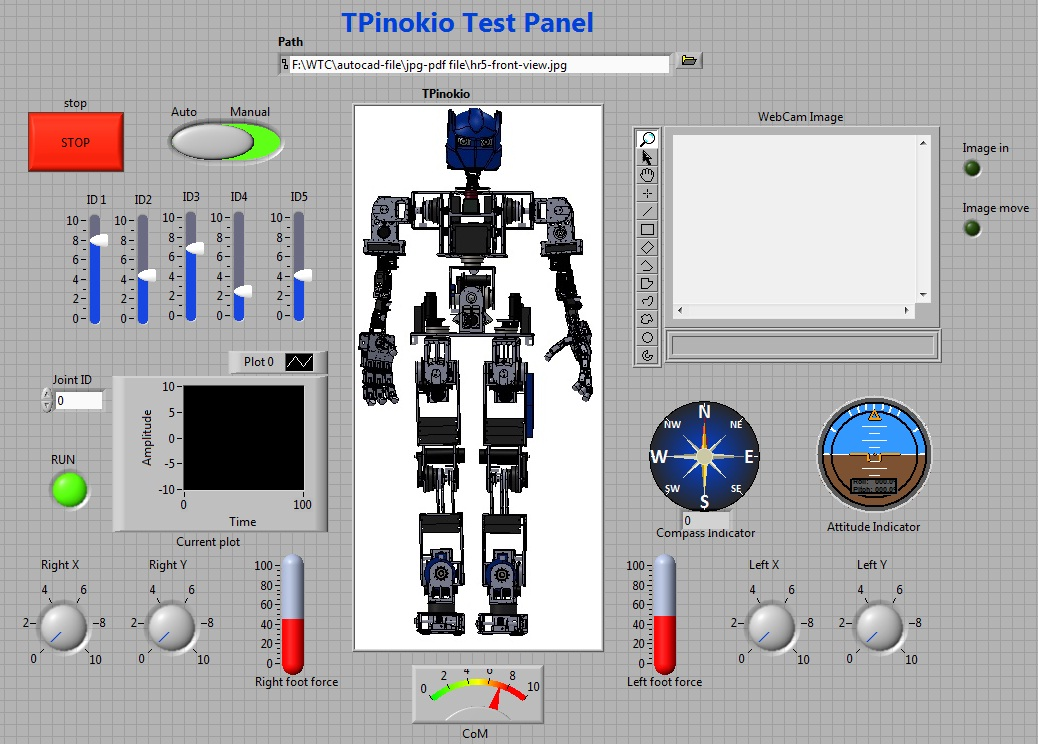
\includegraphics[width=10cm]{CtrlPanel.jpg}
\caption{控制面板} 
\label{fig:xfig1}
\end{figure}

现有的基于动作捕捉的遥操作系统如OptiTrack和机械外骨骼等,虽然用户体验很好,但是成本极高,依赖性强,无法大规模应用;现有的实时VR显示大多基于图像拼接,图像采集设备昂贵,实时性和图像质量无法同时兼顾,且对算力要求很高。

本作品提出了一种廉价、低延时的遥操作系统,其双目摄像头及VR显示系统可使操作者看到具有立体感的实时画面,手持追踪器操作机械臂末端符合人类日常使用手进行操作的习惯,可以给予操作者以身临其境的操作体验。


\chapter{现有系统问题}

\section{现有的三维图像采集系统}

目前三维场景重构需要很高的算力,分辨率低且不能保证实时性,目前较成熟的实时三维场景采集系统基本上都基于图像拼接技术:

\begin{figure}
\begin{minipage}{0.48\textwidth}
  \centering
  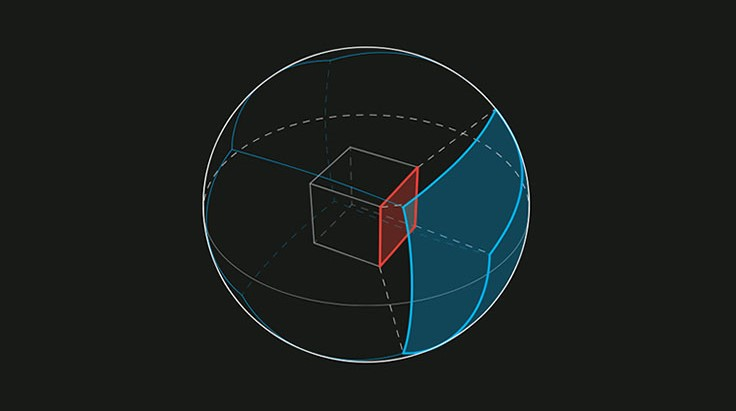
\includegraphics[height=4cm]{Cube.jpg}
  \caption{立方体拼接}
  \label{fig:p1}
\end{minipage}\hfill
\begin{minipage}{0.48\textwidth}
  \centering
  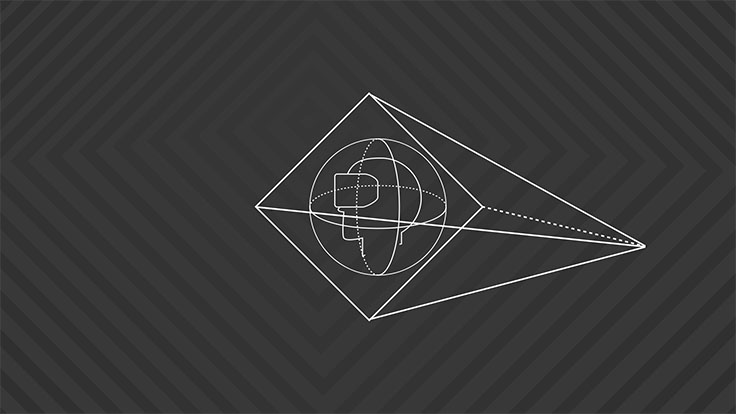
\includegraphics[height=4cm]{Tri.jpg}
  \caption{金字塔形拼接}
  \label{fig:p2}
\end{minipage}
\end{figure}

就图像传输系统而言,要创建一个360度的视频,无论是使用一组特殊的摄像机同时记录360度的场景,还是将4个不同角度的GoPros图像拼接在一起。传入的360度视频文件是4K和更高,比特率可以超过50 Mb/s。而用于VR的3D 360度视频是其两倍,即每小时44 GB视频。如果要实时发送和接收这些图像信息,对带宽等网络环境要求非常高。另外无论采用立方体还是金字塔形拼接方式,拼接这些图像会消耗大量的算力,运算和传输延迟加起来都会达到2s以上,实时性和图像质量无法同时兼顾。

就图像采集设备而言,以Google Jump为例,Google Jump使用24个GoPro,环绕一个圆形分布,考虑到GoPro单个相机的价格(2000-3000人民币)上述系统造价非常昂贵。
\begin{figure}[htbp]
\small
\centering
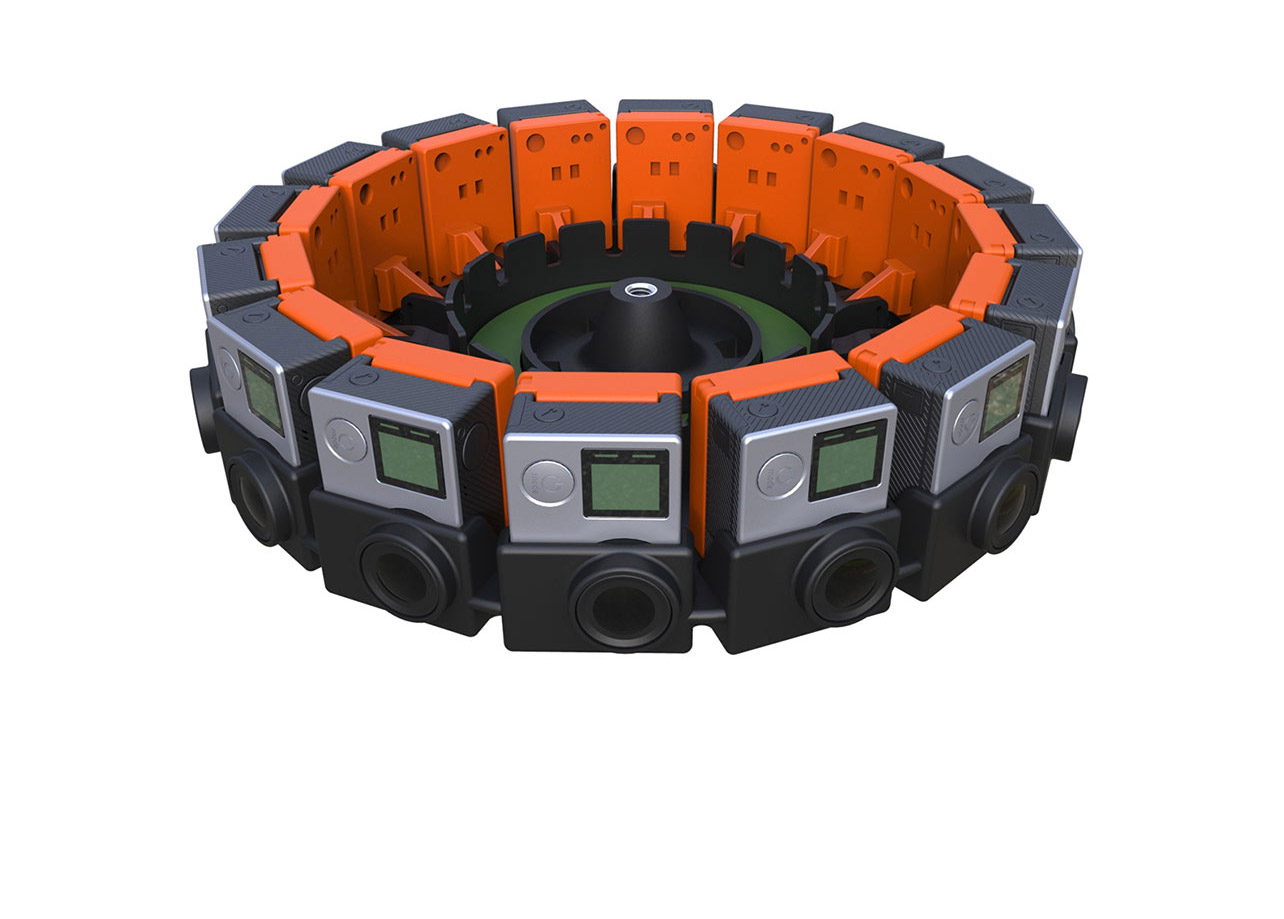
\includegraphics[width=16cm]{google-jump.jpg}
\caption{Google Jump} 
\end{figure}

\section{现有的机器人遥操作系统}
\subsection{计算机指令或手柄控制}
许多需要人工远程操控的机器人,其操作方式基本都是向控制面板或计算机输入指令而实现。工作人员需要熟悉各种操作平台,并需要长时间紧盯电脑屏幕进行操作,其交互体验不是很理想。

另一些用户界面比较友好的机器人使用摇杆控制

\subsection{OptiTrack}
OptiTrack\footnote{\url{http://optitrack.com/}} 是基于一系列红外摄像机的动作捕捉系统解决方案,在操作者身上贴多个感光球,通过四周的十多个红外摄像机来计算每一个感光球的位置,从而获得人的动作数据。
\begin{figure}[H]
\small
\centering
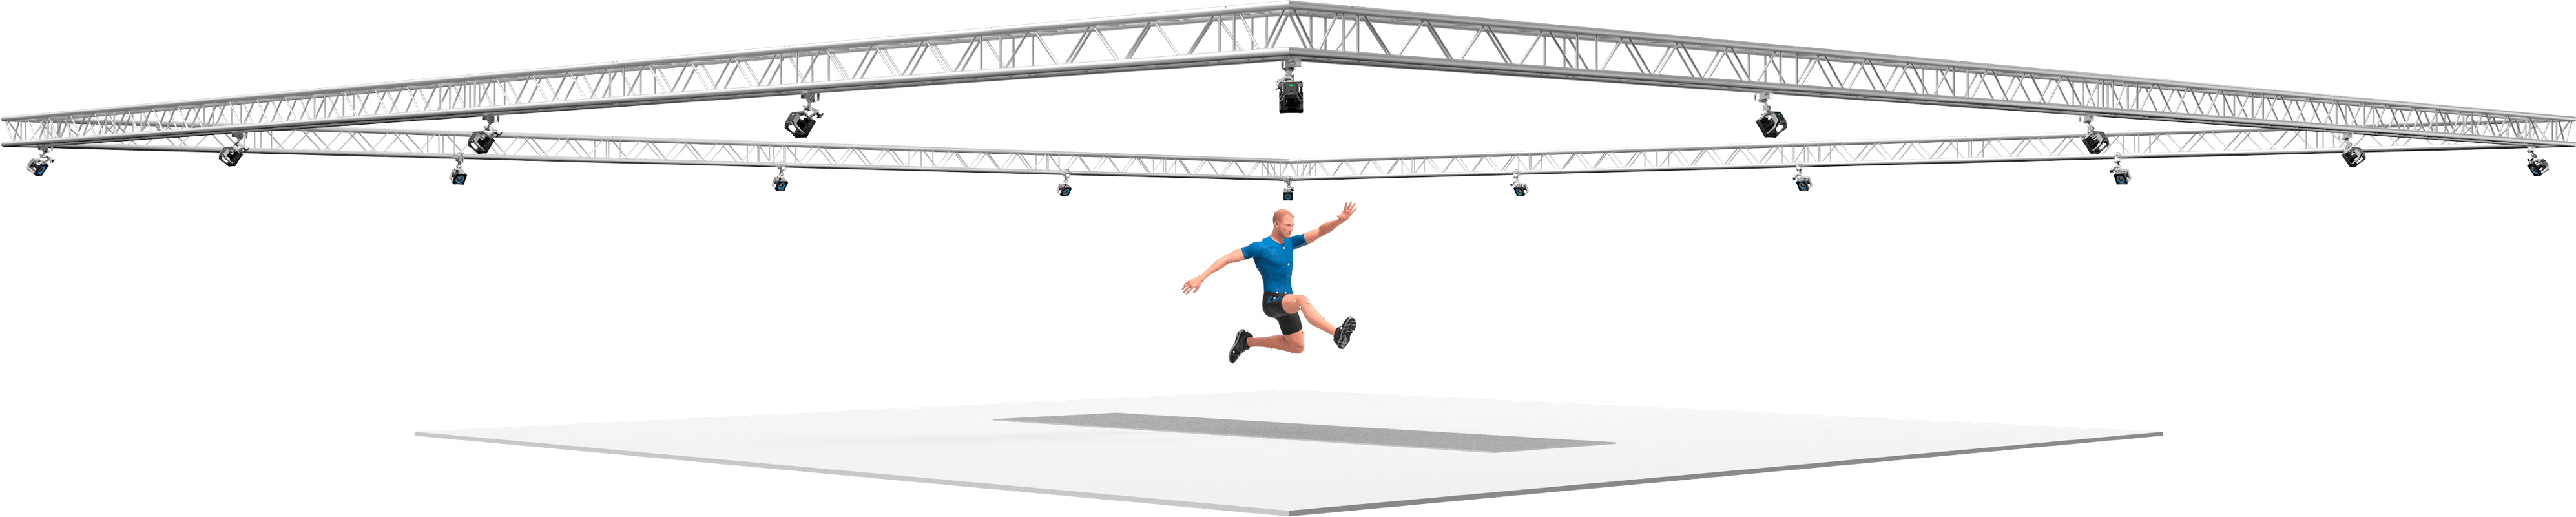
\includegraphics[width=16cm]{movementPrime41_16.png}
\caption{OptiTrack} 
\end{figure}
由于此解决方案需要至少12个高速红外摄像机和配套的处理系统,而一个红外摄像机售价4000-5000美元,整个系统的成本非常高,用其做机器人控制并不现实。

\subsection{T-HR3}

T-HR3是一种远程机动系统,它通过外骨骼和数据手套将手,手臂和脚部动作映射到机器人。

就操作者近端方面而言,T-HR3采用机械外骨骼加上双手的数据手套。由于机械外骨骼以力信号作为控制端的输出信号,所以,机械外骨骼和操作者之间本身就存在一定的滞后性,而且,力信号易受外力干扰,所以存在信号不稳定的问题。

另外,T-HR3需要一套昂贵且笨重的外骨骼,其应用场景十分受限。

\begin{figure}[htbp]
\small
\centering
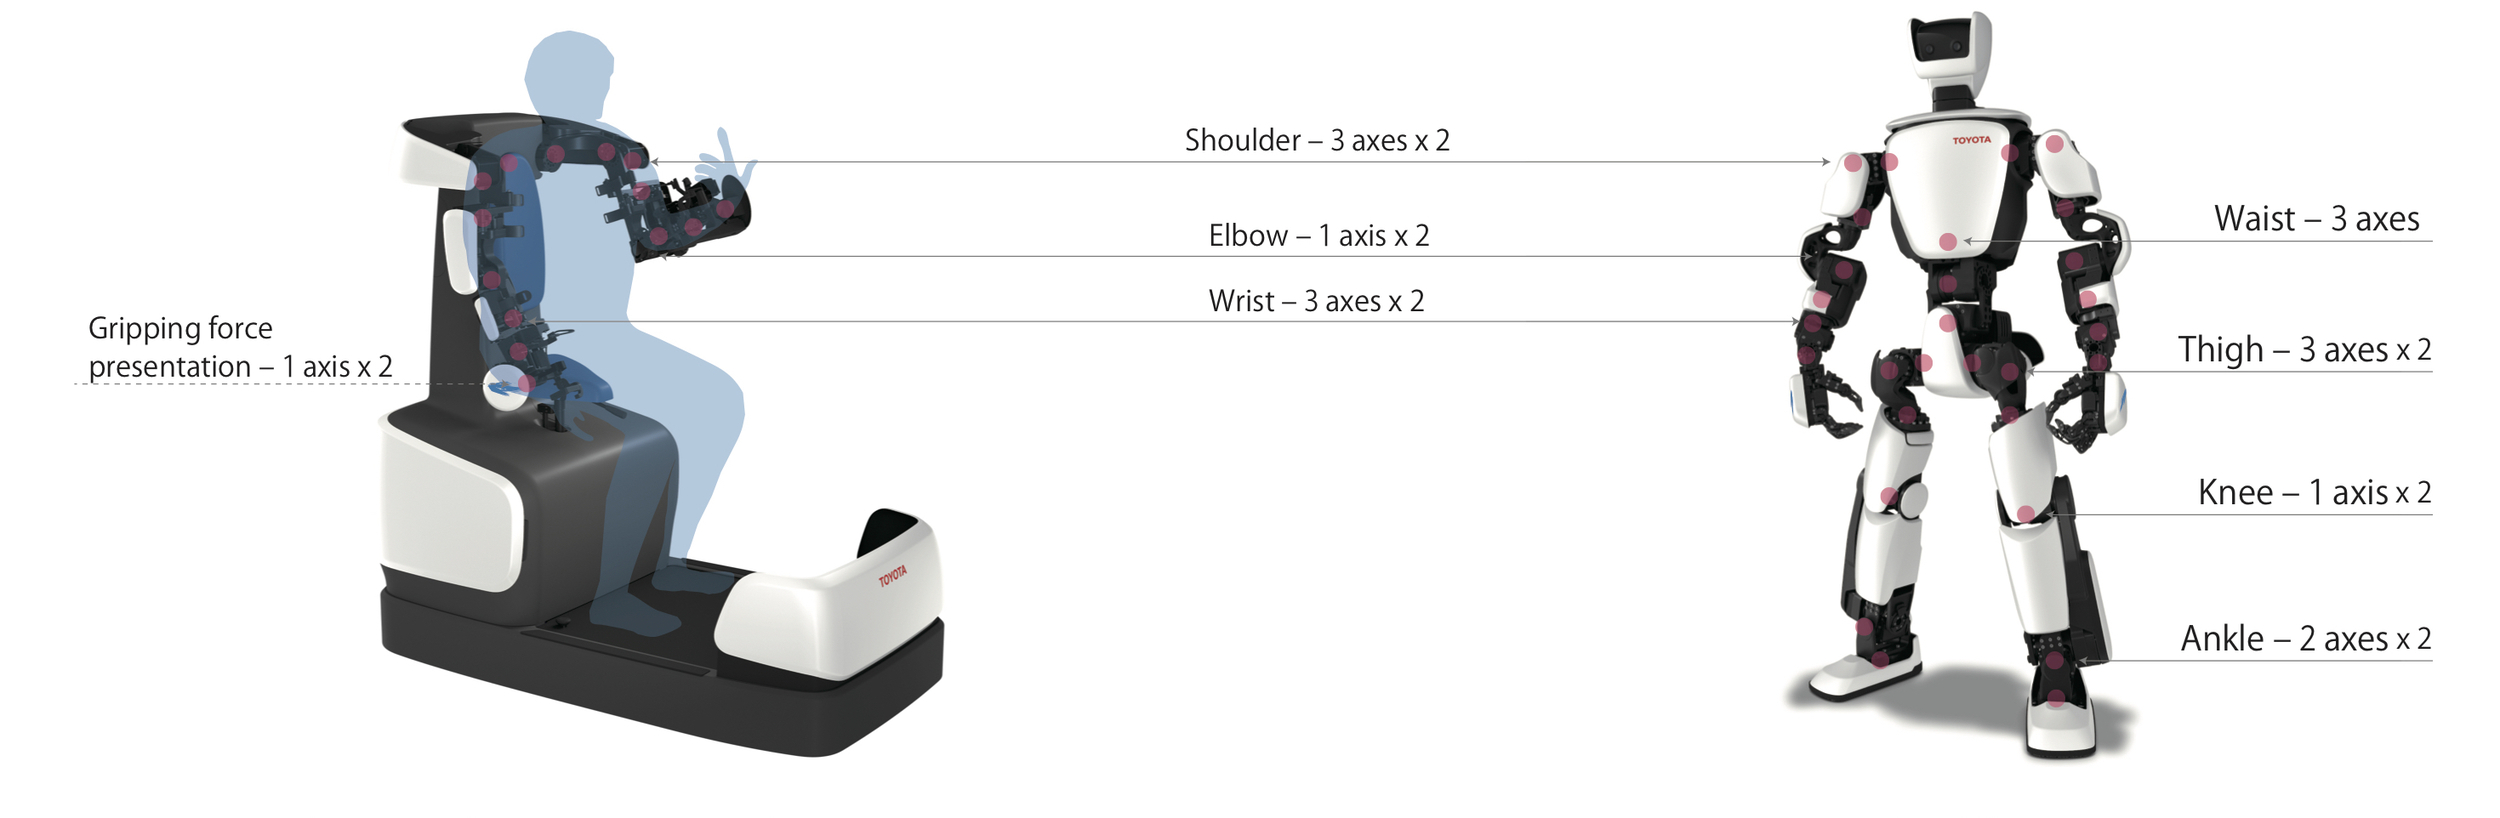
\includegraphics[width=16cm]{T-HR3_2.jpg}
\caption{T-HR3} 
\end{figure}

\chapter{系统简介}

该项目可分为两个子系统:图像显示系统及机器人控制系统。
	
	\section{VR远程监视系统}
本项目旨在提供一个具有较强立体感的实时全景图像,并解决现有系统的问题以及最大化的降低造价,以使远程操控者获得身临其境的体验。我们用ZED双目摄像头来采集实时场景信息,两个目采集到的图像对应到VR眼镜的两个显示屏中,而搭载ZED的多自由度舵机支架可随操纵者头部的转动而实时旋转,以保证双目摄像头的朝向和操作者双眼朝向一致,从而使操作者可以实时地看到各方位的立体场景。
	
此系统硬件部分仅由一个双目摄像头,转台,虚拟现实头盔组成,成本低,且部件较常见。双目摄像头可以由两个独立的摄像头替代,只需保证两摄像头间距和瞳距相似即可,随着虚拟现实技术的发展,分辨率较高的Vive VR头盔价格可以为普通人所接受,Google Cardboard售价低至10RMB,和智能手机配合使用。
\begin{figure}
\begin{minipage}{0.48\textwidth}
  \centering
  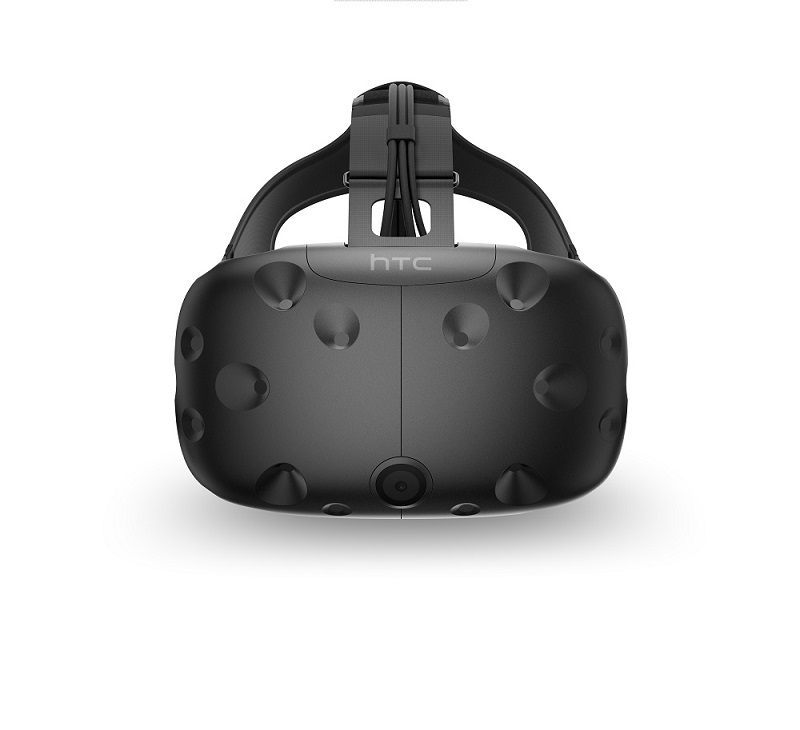
\includegraphics[height=4cm]{HMD.jpg}
  \caption{Vive VR头盔}
  \label{fig:parallel1}
\end{minipage}\hfill
\begin{minipage}{0.48\textwidth}
  \centering
  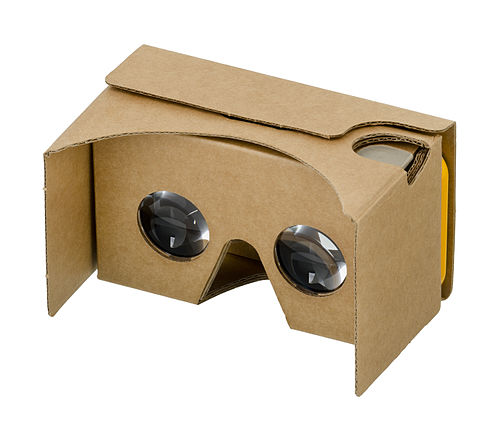
\includegraphics[height=4cm]{Google-Cardboard.jpg}
  \caption{Google Cardboard}
  \label{fig:parallel2}
\end{minipage}
\end{figure}

因为只需要传输两个摄像头的图像,且并不需要复杂的运算,这套机械式的实时全景系统延迟很小。

\section{Vive追踪器遥操作系统}

虚拟现实头盔和追踪器上的红外定位模块精确的确定了它们的绝对位置,由此可得它们的相对位置,我们可以使机械臂末端和双目摄像头的相对位置和其一致,从而实现操作者直接用手的位置来控制机械臂。

此系统使得操作者能够利用自身的动作控制机器人的运动,符合人类的行为习惯,因而会带来良好的操作体验。

Vive虚拟现实套件\footnote{\url{https://www.vive.com/cn/product/}}包括Vive追踪器,Vive VR头盔和Lighting基站,官网售价5488RMB,远低于OptiTrack或T-HR3外骨骼部分的售价。而这套系统完全可以胜任大多数任务。而且Vive VR套件对环境要求很低,可以随时搭建操作环境。
\begin{figure}[H]
\small
\centering
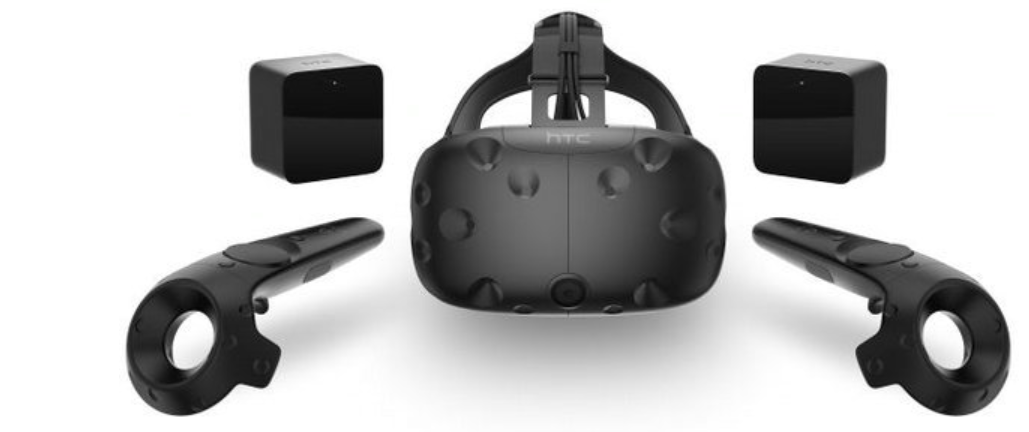
\includegraphics[width=16cm]{vive.PNG}
\caption{Vive虚拟现实套件} 
\end{figure}

\chapter{技术细节}

\section{实时图像采集与显示系统}
项目用于和Vive头盔进行互动的是一个ZED双目摄像头。ZED双目摄像头搭载在由两个数字舵机组成的双自由度平台上,用于与用户交互。

整个系统放置在4轮全向轮底盘上面, ZED双目摄像头采集到的图像,通过USB3.0发送给Nvidia Jetson TX1\footnote{\url{http://www.nvidia.cn/object/embedded-systems-dev-kits-modules-cn.html}},TX1上运行Ubuntu,图像在TX1上处理后,使用UV4L服务(User space Video4Linux)\footnote{\url{https://www.linux-projects.org/uv4l/}}发送到局域网。同时,Vive VR头盔的姿态数据通过HTC串流盒发送到计算机中进行处理,处理后通过蓝牙串口发送到全向轮车上面的Arduino Mega 2560,控制双自由度数字舵机做出与Vive VR头盔同步的转动,使安装在双自由度数字舵机平台上的ZED双目摄像头的指向与Vive头盔实时相同。

演示视频参见附件XXX

\section{机械臂控制系统}

\begin{figure}[htbp]
\small
\centering
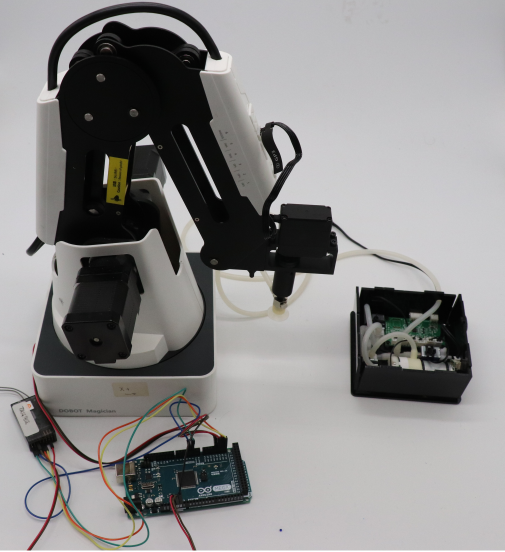
\includegraphics[width=8cm]{Dobot0.png}
\caption{DOBOT机械臂及通讯系统} 
\end{figure}


\section{NAO机器人控制系统}
项目中为了控制机器人的手臂,采用逆运动学的理论,通过机器人手臂的端点结合手臂的参数来计算关节必要的旋转值来进行动作。由于NAO机器人手臂(不包括手指部分)的自由度是5个,因此在仅要设置手指尖端的目标坐标点的情况下,会出现手臂姿态不唯一的情况。通过筛选使得手臂各个关节与端点的坐标实现一一对应。

\begin{figure}[htbp]
\small
\centering
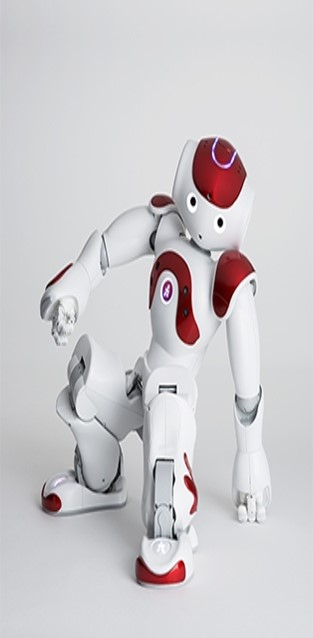
\includegraphics[width=8cm]{NAO.jpg}
\caption{NAO机器人} 
\end{figure}

对于机器人的姿态设定、手臂末端的设定涉及到机器人的控制理论。每个关节有相应的标准坐标系来解读链接和位置以及决定关节转换的基本程序。从参考点开始到第一个关节,再最终到最后一个关节完成转换后可以得到机械臂的转换矩阵。利用这个转换矩阵可以根据手臂末端的目标位置得到每个关节的转动参数。

我们主要采用Denavit Hartenberg (DH)来进行运动学的计算。根据厂家提供的机器人的手臂参数(如长度等),得到每个关节n的转换矩阵$A_n$

\begin{equation}
{{A}_n} = \left[ {\begin{array}{*{20}{c}}
	{{C_{{\theta _n}}}}&{ - {S_{{\theta _n}}}{C_{{\alpha _n}}}}&{{S_{{\theta _n}}}{S_{{\alpha _n}}}}&{{a_n}{C_{{\theta _n}}}}\\
	{{S_{{\theta _n}}}}&{{C_{{\theta _n}}}{C_{{\alpha _n}}}}&{ - {C_{{\theta _n}}}{S_{{\alpha _n}}}}&{{a_n}{S_{{\theta _n}}}}\\
	0&{{S_{{\alpha _n}}}}&{{C_{{\alpha _n}}}}&{{d_n}}\\
	0&0&0&1
	\end{array}} \right]
\end{equation}

其中${C_{{\theta _n}}} = \cos ({\theta _n})$,${S_{{\theta _n}}} = \sin ({\theta _n})$, ${{\theta }_{n}}$为官方给出的旋转角,$a_n$为两个关节参考坐标系中坐标轴交界口的距离,$d_n$为两个关节在同意旋转轴上的距离,这些数据都可以在NAO的数据手册中查询到。

为了根据目的点的坐标分离方程,以得到各个关节的转动值,我们将变换矩阵"An"的逆矩阵相乘于关系方程的左边来取得计算角度值的元素。右手包含五个关节,从上到下分别是肩膀关节(RShoulderPitch,RShoulderRoll 两个),手肘关节(elbow RElbowRoll,RElbowYaw 两个),和手腕关节(RWristYaw)。因此,表示从肩膀到手腕各关节的转动矩阵为${}_{S}^{W}{T}$

\begin{equation}
{}_{s}^{\rm{w}}{T = }{{A}_{1}} \times {{A}_{2}} \times {{A}_{3}} \times {{A}_{4}} \times {{A}_{5}}
\end{equation}

\begin{equation}
	A = {A_1} \times {A_2} \times {A_3} \times {A_4} \times {A_5} = \left[ {\begin{array}{*{20}{c}}
		{{r_{11}}}&{{r_{12}}}&{{r_{13}}}&{{p_x}}\\
		{{r_{21}}}&{{r_{22}}}&{{r_{23}}}&{{p_y}}\\
		{{r_{31}}}&{{r_{32}}}&{{r_{33}}}&{{p_z}}\\
		0&0&0&1
		\end{array}} \right]
\end{equation}

然后我们通过逐步乘以 $ A_i^{-1} $ 的方式得到各个关节的变换矩阵A,进而可以通过以下公式得到每个关节的转动参数。

\begin{equation}
{Pos\_w = A} \times {Pos\_s}
\end{equation}

由以上方程并结合NAO的链接关节变量数据(在NAO官网上提供),我们可以根据目的点得到每个关节点旋转的角度,从而达到基于逆运动学控制机器人的机械臂。



\chapter{项目展示}

现阶段已完成一个由全向轮底盘移动的机械臂,平台上搭载多自由度机械结构托举的双目摄像头,随着操作者头部的转动而同步转动,以采集实时图像信息。

\begin{figure}
\begin{minipage}{0.48\textwidth}
  \centering
  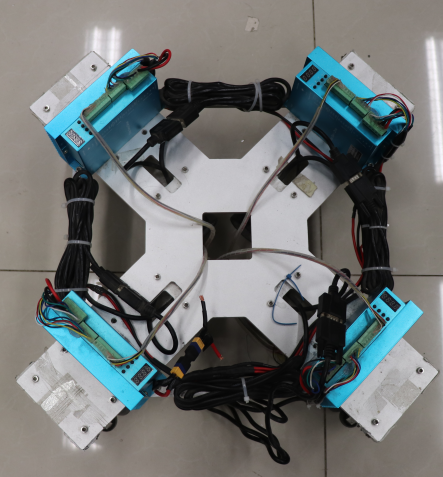
\includegraphics[height=6cm]{car.png}
  \caption{全向轮底盘}
  \label{fig:parallel1}
\end{minipage}\hfill
\begin{minipage}{0.48\textwidth}
  \centering
  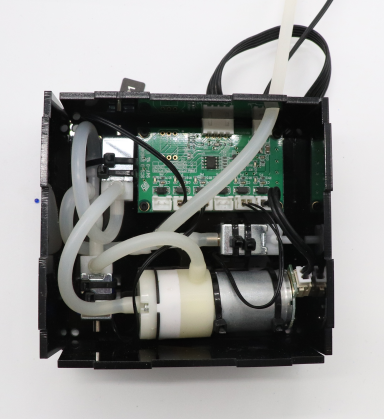
\includegraphics[height=6cm]{bump.png}
  \caption{气泵和电磁阀组建的吸附装置}
  \label{fig:parallel2}
\end{minipage}
\end{figure}

我们可以实现读取追踪器和VR头盔绝对位置并通过串口发送。可以看到图片中输出了左手,右手和头盔的绝对坐标。我们改写了机械臂底层及接口,解决了串口控制卡顿的情况。现在已实现用遥控器-接收机控制系统,远程完成叠纸杯实验。另外,我们在机械臂末端加上了吸盘执行机构,使用气泵和电磁阀组建了一个吸附装置。四轮全向轮底盘也搭建完成。

\begin{figure}[htbp]
\small
\centering
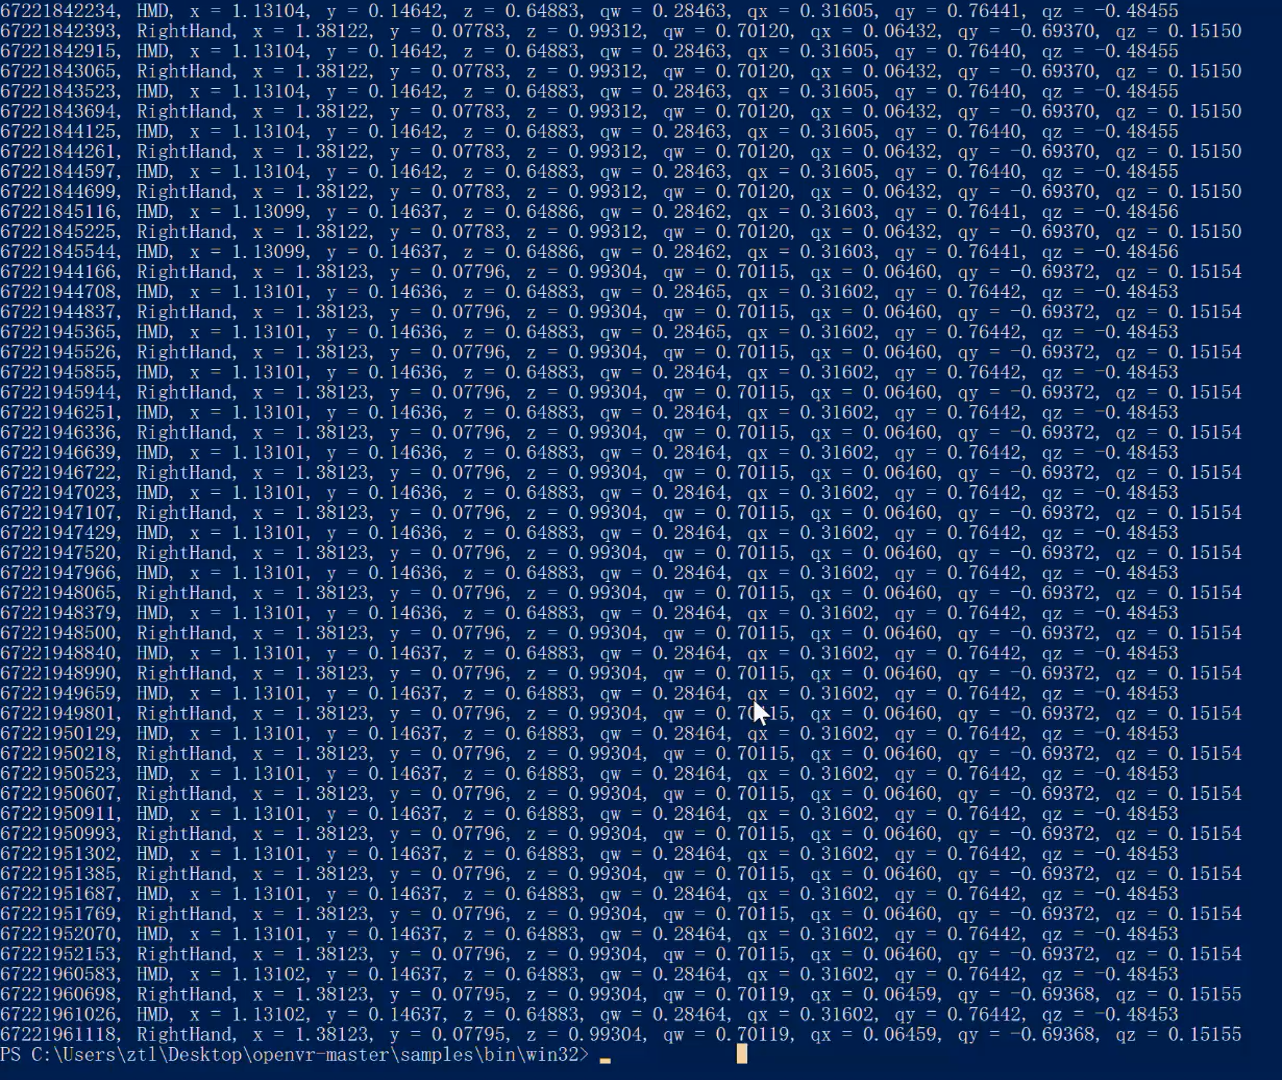
\includegraphics[width=16cm]{Date.png}
\caption{追踪器和VR头盔绝对位置} 
\end{figure}

经测试,我们这套系统远程控制实时性很好,视频传输感受不到延迟,在VR眼睛中有很强的立体感。此外,控制较传统方式更简便,追踪器较外骨骼造价低。

在之后的一段时间内,我们将调用追踪器位置信息,发送给下位机,实现追踪器控制机械臂的功能。

另外我们刚刚借到了Now机器人,准备在操作者手脚上放置四个追踪器,以此来控制机器人的运动,如站立,行走等。


\chapter{未来应用}
未来此技术可以用于拆弹,救援,远程交互等领域。为了完善机器人的功能,可以加上手势识别元件实现机器人手部的动作。

此外,该系统中机器人可不断对操控者的行为进行学习。通过采集每次操作的数据,可以使用增强学习训练机器人自主地执行任务。


%% 参考文献
% 注意:至少需要引用一篇参考文献,否则下面两行可能引起编译错误。
% 如果不需要参考文献,请将下面两行删除或注释掉。
% 数字式引用
\bibliographystyle{thuthesis-numeric}
% 作者-年份式引用
% \bibliographystyle{thuthesis-author-year}
\bibliography{ref/refs}

\end{document}
